%!TEX TX-program = xelatex
\documentclass[8pt]{article}

\usepackage{ctex}
\usepackage{graphicx}
\usepackage{enumitem}
\usepackage{geometry}
\usepackage{amsmath}
\usepackage{amssymb}
\usepackage{amsfonts}
\usepackage{tikz}
\usepackage{extarrows}
\usetikzlibrary{positioning}
\usetikzlibrary{svg.path}
\usepackage{xcolor}
\usepackage{soul}
\usepackage{longtable}

\graphicspath{ {./images/} }

\title{5 函数的概念、性质及应用}
\author{高一(6)班\ 邵亦成\ 26号}
% \date{2021年11月??日}

\geometry{a4paper, scale=0.8}

\setcounter{section}{4}

\begin{document}

	\maketitle

	\section{函数的概念、性质及应用}
		\subsection{函数}
			\textbf{函数的定义}: 设$D$是一个\textbf{非空的实数集}, 如果按照某种\textbf{确定的对应关系$f$}, 使对集合$D$中的\textbf{任意给定的$x$}, 都有\textbf{唯一的实数$y$}与之对应, 就称这个对应关系$f$为集合$D$上的一个\textbf{函数}, 记作$$y=f(x), x \in D.$$ 其中, $x$叫做\textbf{自变量}, 其取值范围 (数集$D$) 称为该函数的\textbf{定义域}. 

			此时,就称$y$是$x$的函数, 当自变量$x$取值$x_0$时, 由对应关系$f$所确定的对应于$x_0$的值$y_0$, 称为函数在$x_0$处的\textbf{函数值}, 记作$y_0=f(x_0)$.

			所有函数值组成的集合$\{y|y=f(x), x\in D\}$称为这个函数的\textbf{值域}.

			对应关系常用小写字母$f, g, h$等来表示.

			\textbf{函数的三要素}: 定义域, 对应关系, 值域.

			\textbf{函数的三要素之间的关系}: 定义域 and 对应关系 $\Rightarrow$ 值域; 定义域 and 值域 $\nRightarrow$ 对应关系; 值域 and 对应关系 $\nRightarrow$ 定义域.

			\textbf{两个函数相同}: 定义域与对应关系完全一致.
			~\\

			\textbf{函数的表示方法}: 列表法, 解析法, 图像法.

			\textbf{列表法}: 通过列出自变量的值与对应函数值的相应表格来表达函数关系的方法称为\textbf{列表法}. 列表法通常用在定义域为有限集的情况.

			\textbf{解析法}: 用一个数学表达式来表示两个变量之间的对应关系, 这种表示函数的方法称为\textbf{解析法}.

			\textbf{分段表示法}: 有一些函数在不同的区间上可以有不同的表达式. 例如,函数$y=|x|$就是通过

			$$
			y=
			\left\{
			\begin{array}{rl}
			x,&x\geq 0,\\
			-x,&x<0
			\end{array}
			\right.
			$$

			来定义的. 这样表示函数的方法叫做\textbf{分段表示法}. 分段表示法也是一种解析法.

			注意分段函数的定义域是几段的并集, 且最值只有一个.

			\textbf{图像法}: 利用函数的图像来表示图像的方法称为\textbf{图像法}.

			\textbf{图像}: 对于函数$y=f(x), x\in D$, 其定义城$D$中每一个$x$的值都有唯一的一个$y$值与之对应. 把这两个对应的数构成的有序实数对$(x, y)$作为点$P$的坐标, 记作$P(x, y)$. 所有这些点组成的集合$G$叫做函数$y=f(x), x\in D$的图像, 即

			$$
			G=\{(x, y)|y=f(x), x\in D\}.
			$$

			如果对定义城$D$中的实数$x_0$, 有$f(x_0)=y_0$, 那么点$P(x_0, y_0)$一定在该函数的图像上; 反之, 如果点$P(x_0, y_0)$在该函数的图像上, 那么必有$x\in D$,且$y_0=f(x_0)$.

			~\\

			\textbf{例一}: $f(x+1)=x^2-3x+2, x\in [1, 2]$. 求$f(x), f(x-1).$
				~\\

				令$t=x+1$, 则$x=t-1$.

				$f(t)=t^2-5t+6, t\in[2, 3].$

				$f(x)=x^2-5x+6, x\in[2, 3].$

				$f(x-1)=(x-1)^2-5(x-1)+6=x^2-7x+12, x-1\in[2, 3]\text{ 即 }x\in[3, 4].$

				\textbf{\textcolor{red}{总结: 复合函数使用换元是一个相当不错的方法, 换元须注意元的取值范围.}}

			~\\

			\textbf{例二}: 求$\displaystyle \frac{\sqrt{|x-3|-2} \cdot (x-1)^0}{x+|x|}$的定义域.
				~\\

				$$
				\left\{
				\begin{array}{rclcrcl}
					|x-3|-2&\geq&0&\Rightarrow&x&\in&(-\infty, 1]\cup[5, +\infty)\\
					x-1&\neq&0&\Rightarrow&x&\neq&1\\
					x+|x|&\neq&0&\Rightarrow&x&>&0\\
				\end{array}
				\right.
				\Rightarrow
				x\in(0, 1)\cup[5, +\infty).
				$$

				\textbf{\textcolor{red}{总结: 非实际问题的定义域即为使该式有意义的$x$的取值范围, 一般限定条件为根号, 0次方, 分母等.}}

			~\\

			\textbf{抽象函数 (复合函数) 的定义域}: $f(g(x))=f \circ g (x)$的定义域$D$指$x$的取值范围, 即$D_{g}$. 此时同时有$R_{g}=D_{f}.$

			~\\

			\textbf{例三}: 若$f(x^2)$的定义域是$[1, 3]$, 求函数$f(x+1)$的定义域.
				~\\

				$x\in [1, 3] \Rightarrow x^2 \in [1, 9] \Rightarrow D_{f}=[1, 9] \Rightarrow x+1\in[1, 9] \Rightarrow x\in[0, 8] \Rightarrow D_{f(x+1)}=[0, 8].$

				\textbf{\textcolor{red}{总结: 求定义域使用换元也十分有用.}}

			~\\

			\textbf{例四}: 函数$f(x)$有

				$$
				\left\{
				\begin{array}{rl}
				x^2+2x,&x\geq 0,\\
				-x^2-2x,&x<0.
				\end{array}
				\right.
				$$

				\begin{enumerate}[label=(\arabic*)]
					\item 求方程$f(x)=1$的解.
					\item 计算满足$f(-a)=f(a)$的实数$a$.
					\item 试根据$a$的取值讨论方程$f(x)=a$的根的个数问题.
				\end{enumerate}
				~\\

				\begin{enumerate}[label=(\arabic*)]
					\item 求方程$f(x)=1$的解.

						分两类讨论.

						\begin{enumerate}[label=$\arabic*^{\circ}$]
							\item $x\geq 0 \Rightarrow x^2+2x=1 \Rightarrow x=-1\pm \sqrt {2} $(舍负).

							\item $x < 0 \Rightarrow -x^2-2x=1 \Rightarrow x=-1.$
						\end{enumerate}

						综上, 解为$x_1=-1+\sqrt{2}, x_2=-1.$

					\item 计算满足$f(-a)=f(a)$的实数$a$.

						分三类讨论.

						\begin{enumerate}[label=$\arabic*^{\circ}$]
							\item $a > 0 \Rightarrow a^2+2a=-a^2+2a \Rightarrow a=0$(舍).

							\item $a = 0 \Rightarrow f(a)=f(-a)=f(0)=0.$

							\item $a < 0 \Rightarrow a^2-2a=-a^2-2a \Rightarrow a=0$(舍).
						\end{enumerate}

						综上, $a=0.$

					\item 试根据$a$的取值讨论方程$f(x)=a$的根的个数问题.

						$$
						\begin{tikzpicture}[scale=0.5]
				    		\draw[black, ->] (-5, 0)--(5, 0) node[anchor=north] at (5, 0) {$x$};
				    		\draw[black, ->] (0, -5)--(0, 5) node[anchor=east] at (0, 5) {$y$};
				    		\draw[black, domain=-3:0] plot(\x, -\x*\x-2*\x) node[anchor=north west] at (0, 0) {$O$};
				    		\draw[black, domain=0:3] plot(\x, 0.5*\x*\x+\x);
				    		\filldraw[black] (-2, 0) circle (2pt) node[anchor=south east] {$-2$};
				    		\draw[black, dashed] (-1, 1)--(0, 1) node[anchor=south east] at (0, 1) {$1$};
						\end{tikzpicture}
						$$

						根的个数即$y=f(x)$与$y=a$的图像的交点.

						$a<0$或$a>1$时, 一解; $a=0$或$a=1$时, 两解; $0<a<1$时, 三解. 

				\end{enumerate}

				\textbf{\textcolor{red}{总结: 使用函数图像的相交判断方程的解的个数是一个十分便捷的方法, 一般多用于直线和曲线/直线和直线, 不常用于曲线和曲线.}}

			~\\

			\textbf{例五}: 函数$f(x)$对于任意实数$f(x)$满足条件:

				$$f(x+2)=\frac{1}{f(x)},$$

				且有$f(0)=1, f(1)=-5.$

				\begin{enumerate}[label=(\arabic*)]
					\item 计算$f(2), f(4), f(6), f(8)$的值, 并猜想$f(2n)$的结果, 其中$n \in \mathbb{N}.$
					\item 计算$f(3), f(5), f(7), f(9)$的值, 并猜想$f(2n-1)$的结果, 其中$n \in \mathbb{N}.$
					\item 试证明(1), (2)所猜想的结果.
				\end{enumerate}
				~\\

				\begin{enumerate}[label=(\arabic*)]
					\item 计算$f(2), f(4), f(6), f(8)$的值, 并猜想$f(2n)$的结果, 其中$n \in \mathbb{N}.$

						$$f(2)=\frac{1}{f(2-2)}=\frac{1}{f(0)}=\frac{1}{1}=1, f(4)=\frac{1}{f(4-2)}=\frac{1}{f(2)}=\frac{1}{1}=1,$$

						$$f(6)=\frac{1}{f(6-2)}=\frac{1}{f(4)}=\frac{1}{1}=1, f(8)=\frac{1}{f(8-2)}=\frac{1}{f(6)}=\frac{1}{1}=1,$$

						猜想:

						$$f(2n)=1, n \in \mathbb{N}. \eqno{(1)}$$

					\item 计算$f(3), f(5), f(7), f(9)$的值, 并猜想$f(2n-1)$的结果, 其中$n \in \mathbb{N}.$

						$$f(3)=\frac{1}{f(3-2)}=\frac{1}{f(1)}=\frac{1}{-5}=-\frac{1}{5}, f(5)=\frac{1}{f(5-2)}=\frac{1}{f(3)}=\frac{1}{-\frac{1}{5}}=-5,$$

						$$f(7)=\frac{1}{f(7-2)}=\frac{1}{f(5)}=\frac{1}{-5}=-\frac{1}{5}, f(9)=\frac{1}{f(9-2)}=\frac{1}{f(7)}=\frac{1}{-\frac{1}{5}}=-5,$$

						猜想:

						$$f(2n-1)=
						\left\{
						\begin{array}{rl}
						-5,& n\text{是奇数},\\
						\displaystyle -\frac{1}{5}, &n\text{是偶数}.\\
						\end{array}
						\right.
						\eqno{(2)}
						$$

					\item 试证明 (1), (2) 所猜想的结果.

						\textbf{下证 (1) 式成立:}

							考虑$n=0$, 有

							$$f(2\times0)=f(0)=1$$

							符合 (1) 式.

							假设 (1) 式对$n=k$成立, 下证其对$n=k+1$成立.

							$$f[2(k+1)]=f(2k+2)=\frac{1}{f(2k+2-2)}=\frac{1}{f(2k)}=\frac{1}{1}=1$$

							成立.

							由第一数学归纳法, (1) 式成立.

						\textbf{下证 (2) 式成立:}

							考虑$n=0$, 有

							$$f(1)=\frac{1}{f(1-2)}=\frac{1}{f(-1)}=\frac{1}{f(2\times 0-1)}=-5 \Rightarrow f(2\times0-1)=f(-1)=-\frac{1}{5}$$

							符合 (2) 式.

							考虑$n=1$, 有

							$$f(2\times 1-1)=f(1)=-5$$

							符合 (2) 式.

							假设 (2) 式对$n=2k$成立, 下证其对$n=2k+2$成立.

							$$f[2(2k+2)-1]=f(4k+3)=\frac{1}{f(4k+3-2)}=\frac{1}{f(4k+1)}=\frac{1}{\frac{1}{f(4k+1-2)}}=\frac{1}{\frac{1}{f(4k-1)}}=f(4k-1)=f[2(2k)-1]=-\frac{1}{5}$$

							成立.

							假设 (2) 式对$n=2k+1$成立, 下证其对$n=2k+3$成立.

							$$f[2(2k+3)-1]=f(4k+5)=\frac{1}{f(4k+5-2)}=\frac{1}{f(4k+3)}=\frac{1}{\frac{1}{f(4k+3-2)}}=\frac{1}{\frac{1}{f(4k+1)}}=f(4k+1)=f[2(2k+1)-1]=-5$$

							成立.

							由第一数学归纳法, (2) 式成立.

							\textbf{使用周期函数证明}:

							$$f(n+4)=f[(n+2)+2]=\frac{1}{f(n+2)}=f(x),$$

							即该函数存在周期$T=4$.

							又$\because f(0)=1, f(1)=-5, f(-1)=\displaystyle-\frac{1}{5}$

							$\therefore$......得证.
				\end{enumerate}

				\textbf{\textcolor{red}{总结: (1) $\displaystyle f(x+k)=\frac{1}{f(x)} \Rightarrow $周期$T=2k$ (2) 周期法证明和数学归纳法证明都是十分有效的方案.}}

		\newpage
		\subsection{函数的性质}
			\subsubsection{函数的奇偶性}
				\textbf{函数是奇函数或偶函数的前提}: 函数的定义域$D$关于原点对称, 即$\forall x\in D: -x\in D$.

				\textbf{偶函数的定义}: 对于函数$y=f(x)$, 如果\textbf{对其定义域$D$中任意给定的元素$x$, 都有$-x\in D$, 并且$f(-x)=f(x)$}, 就称函数$y=f(x)$为\textbf{偶函数}.

				\textbf{偶函数的图像}: 偶函数就是\textbf{其图像关于$y$轴对称}的函数.

				\textbf{奇函数的定义}:  对于函数$y=f(x)$, 如果\textbf{对其定义域$D$中任意给定的元素$x$, 都有$-x\in D$, 并且$f(-x)=-f(x)$}, 就称函数$y=f(x)$为\textbf{奇函数}.

				\textbf{奇函数的图像}: 奇函数就是\textbf{其图像关于原点中心对称}的函数.

				\textbf{证明函数是偶函数/奇函数}: (1) $\forall x\in D_f: -x\in D_f$ (2) $\forall x\in D_f: f(-x)=(-)f(x)$.

				\textbf{证明函数不是偶函数/奇函数}: $\exists x\in D_f: -x\notin D_f$ or $\exists x\in D_f: f(-x)\neq (-)f(x)$.

				\textbf{既是奇函数又是偶函数的函数}: $f(x)=0, \displaystyle x\in\bigcup_{x\in A, A \subseteq \mathbb{R}} \left\{x, -x\right\}.$

				\textbf{证明函数既不是奇函数也不是偶函数}: $\exists x\in D_f: -x\notin D_f$ or $\exists x\in D_f: f(-x)\neq \pm f(x)$.

				\textbf{偶/奇函数性质的意义}: 通过$x\geq 0 / x\leq 0$部分的性质推出其在另一部分的性质.

				\textbf{偶/奇函数的加 (减)}: 偶$+$偶$=$偶; 奇$+$奇$=$奇.

				\textbf{偶/奇函数的乘 (除)}: 偶$\times$偶$=$偶; 奇$\times$奇$=$偶; 偶$\times$奇$=$奇.

				~\\

				\textbf{例一}: 证明: $f(x)=x^6+2x^4-3|x|$是偶函数.
					~\\

					定义域$D=\mathbb{R}$, 满足$\forall x\in D: -x \in D$.

					考虑$x\in D=\mathbb{R}$,

					$f(-x)=(-x)^6+2\cdot (-x)^4-3|(-x)|=x^6+2x^4-3x=f(x)$.

					即$f(x)=x^6+2x^4-3|x|$是偶函数.

					\textbf{\textcolor{red}{总结: 证明偶函数的方法: (1) $\forall x\in D_f: -x\in D_f$ (2) $\forall x\in D_f: f(-x)=f(x)$.}}

				~\\

				\textbf{例二}: 已知: $f(x)$是偶函数, 当$x\in[-6, -1]$有$f(x)=(x+5)^2-4$. 求: $x\in[1, 6]$时$f(x)$的解析式.
					~\\

					$\forall x\in[1, 6]: -x\in[-6, -1].$

					$f(x)=f(-x)=[(-x)+5]^2-4=x^2-10x+21.$

					\textbf{\textcolor{red}{总结: 利用函数奇偶性求函数解析式的方法注意$x$和$-x$的取值范围.}}

				~\\

				\textbf{例三}: 已知: $f(x)=x^2+bx+c$是偶函数. 求: $b, c$的取值范围.
					~\\

					$f(-x)=(-x)^2+b\cdot(-x)+c=x^2-bx+c=f(x)=x^2+bx+c$对任意$x\in\mathbb{R}$恒成立.

					有$b=0, c\in\mathbb{R}$.

					\textbf{\textcolor{red}{总结: 两个式子若对任意自变量恒相等则有对应系数相等.}}

				~\\

				\textbf{例四}: $f(x)$为奇函数, $g(x)$为偶函数, $f(x)-g(x)=\dfrac{1}{x^2+x} (x\neq 0, 1, -1)$. 求$f(x), g(x)$的解析式.
					~\\

					考虑$x=x, x=-x$有

					$$
					\left\{
					\begin{array}{rcl}
						f(x) - g(x) &=& \dfrac{1}{x^2+x}\\\\
						f(-x) - g(-x) &=& \dfrac{1}{(-x)^2+(-x)}\\
					\end{array}
					\right..
					$$

					又有

					$$f(-x) = -f(x), g(-x) = g(x),$$

					于是有

					$$
					\left\{
					\begin{array}{rcl}
						f(x) - g(x) &=& \dfrac{1}{x^2+x}\\\\
						-f(x) - g(x) &=& \dfrac{1}{(-x)^2+(-x)}\\
					\end{array}
					\right.
					\Rightarrow
					\left\{
					\begin{array}{rcl}
						f(x) &=& ...\\
						g(x) &=& ...\\
					\end{array}
					\right..
					$$

					\textbf{\textcolor{red}{总结: 与“对称性”相关的题可以考虑代入$x=x, x=-x$联立求解.}}

				~\\

				\textbf{例五}: $f(x)$是$\mathbb{R}$上的奇函数, 当$x\in [0, +\infty)$时, $f(x)=x^2+x+a$. 求$f(x)$的解析式.
					~\\

					\textbf{\textcolor{red}{错误示范:}}

					考虑$x\in(-\infty, 0]$, $-x \in [0, +\infty)$, $f(-x)=(-x)^2+(-x)+a=-f(x) \Rightarrow f(x)=-x^2+x-a$.

					\textbf{正确做法:}

					$\because f(x)$是$\textbf{R}$上的奇函数

					$\therefore f(0)=0$

					$\therefore a=0$.

					当$x\in[0, +\infty)$时, $f(x)=x^2+x$.

					令$x\in(-\infty, 0)$, 则$-x\in(0, +\infty)$.

					$f(-x) = (-x)^2 + (-x) = x^2 - x = -f(x)$

					$\therefore f(x)=-x^2+x.$

					综上, $\displaystyle f(x)=\left\{\begin{array}{rl}x^2+x, &x\in[0, +\infty),\\-x^2+x, &x\in(-\infty, 0).\end{array}\right.$

					~\\

					\textbf{变式}: $f(x)$是$\mathbb{R}$上的奇函数, 当$x\in (0, +\infty)$时, $f(x)=x^2+x+a$. 求$f(x)$的解析式.
					~\\

					\textcolor{red}{$a$解不出 (0不在已知解析式内)}.

					$\because f(x)$是$\textbf{R}$上的奇函数

					$\therefore f(-x)=f(x), f(0)=0$

					当$x\in(0, +\infty)$时, $f(x)=x^2+x$.

					令$x\in(-\infty, 0)$, 则$-x\in(0, +\infty)$.

					$f(-x) = (-x)^2 + (-x) = x^2 - x = -f(x)$

					$\therefore f(x)=-x^2+x.$

					综上, $\displaystyle f(x)=\left\{\begin{array}{rl}x^2+x, &x\in(0, +\infty),\\0, &x=0,\\-x^2+x, &x\in(-\infty, 0).\end{array}\right.$

					\textbf{\textcolor{red}{总结: 求奇函数勿忘$f(0)=-f(0)=0$.}}

				~\\

				\textbf{例六}: $f(x) = \left\{\begin{array}{rl}-x^2+x,& x<0,\\ x^2+x, &x>0.\end{array}\right.$ 求证: $f(x)$为奇函数.
					~\\

					$D_f = (-\infty, 0)\cup(0, +\infty)$关于原点对称.

					令$x\in(0, +\infty)$, 则$-x\in(-\infty, 0)$,

					$\therefore f(x)=x^2+x, f(-x)=-(-x)^2+(-x)=-x^2-x,$

					$\therefore \forall x\in(0, +\infty), f(x)=-f(-x).$

					令$x\in(-\infty, 0)$, 则$-x\in(0, +\infty)$,

					$\therefore f(x)=-x^2+x, f(-x)=(-x)^2+(-x),$

					$\therefore \forall x\in(-\infty, 0), f(x)=-f(-x).$

					综上, $f(x)$为奇函数.

					\textbf{\textcolor{red}{总结: 分段函数的奇偶性证明需证明所有的区间, 无论是否对称.}}

				~\\

				\textbf{例七}: 已知$f(x+y)+f(x-y)=2f(x)f(y)$对一切$x, y$成立, 且$f(0)\neq 0$. 求证: $f(x)$是偶函数.
					~\\

					令$x=y=0,$ 有

					$$f(0)+f(0)=2f(0)f(0).$$

					$$\because f(0) \neq 0 \therefore f(0) = 1.$$

					令$x=0,$ 有

					$$f(y)+f(-y)=2f(0)f(y),$$

					$\therefore f(-y)=f(y)$

					$\therefore f(x)$是偶函数.

					\textbf{\textcolor{red}{总结: 出现“带字母恒成立”问题可使用赋值法 (一般可代入$0, 1, -1$).}}

			\subsubsection{函数的单调性}
				\textbf{单调性的定义}: 对于定义在$D$上的函数$y=f(x)$, 设区间$I$是$D$的一个子集. 对于区间$I$上的任意给定的两个自变量的值$x_1, x_2$, 当$x_1 < x_2$时, 如果总有$$f(x_1)\leq f(x_2),$$就称函数$y=f(x)$在区间$I$上是\textbf{增函数}; 而如果总有$$f(x_1)\geq f(x_2),$$就称函数$y=f(x)$在区间$I$上是\textbf{减函数}.

				特别地, 如果总有$$f(x_1) > f(x_2),$$就称函数$y=f(x)$在区间$I$上是\textbf{严格增函数}; 而如果总有$$f(x_1) < f(x_2),$$就称函数$y=f(x)$在区间$I$上是\textbf{严格减函数}.

				“严格增”“严格减”“增”及“减”统为函数的\textbf{单调性}.\\

				\textbf{单调函数、单调区间的定义}: 如果函数$y=f(x)$在某个区间$I$上是增 (减) 函数, 那么就称函数$y=f(x)$在区间$I$上是\textbf{单调函数}, 并称区间$I$是函数$y=f(x)$的一个\textbf{单调区间}.

				一般来说, 所讨论的单调区间总是指满足这一要求的“最大”的单调区间.\\

				\textbf{单调区间的“和”与“$\cup$”}: “和”表示\textbf{两端分别单调}, “$\cup$”表示一个集合.

				\textbf{判定单调性}: (1) 设$x_1, x_2 \in I, x_1 > x_2$, (2) 求$f(x_1)-f(x_2)$, (3) 判定$f(x_1)-f(x_2)$与$0$的关系, (4) 根据定义写出结论.

				~\\

				\textbf{例一}: 证明函数$f(x)=x^2-\dfrac{1}{x^2}$在$(-\infty, 0)$上是严格减函数.
					~\\

					令$x_1, x_2 \in (-\infty, 0), x_1 > x_2$,

					\begin{align*}
						f(x_1)-f(x_2) &= x_1^2 - x_2^2 - \frac{1}{x_1^2} + \frac{1}{x_2^2}\\
						&= (x_1^2 - x_2^2) \left(1+\frac{1}{x_1^2 x_2^2}\right)\\
						&= (x_1 + x_2) (x_1 - x_2) \left(1+\frac{1}{x_1^2 x_2^2}\right).\\
					\end{align*}

					$\because x_2 < x_1 < 0 \therefore x_1 + x_2 < 0, x_1 - x_2 > 0, 1+\dfrac{1}{x_1^2 x_2^2} > 0,$

					$\therefore f(x_1) - f(x_2) < 0$

					$\therefore f(x)$在$(-\infty, 0)$上是严格减函数.

					\textbf{\textcolor{red}{总结: (1)证明函数单调性: (1) 设$x_1, x_2 \in I, x_1 > x_2$, (2) 求$f(x_1)-f(x_2)$, (3) 判定$f(x_1)-f(x_2)$与$0$的关系, (4) 根据定义写出结论. (2) 判断正负需要因式分解判断每个因式的正负.}}

				~\\

				\textbf{例二}: 讨论$f(x)=\dfrac{ax}{x^2-1} (-1<x<1) (a\neq 0)$的单调性.
					~\\

					令$-1<x_2<x_1<1$,

					\begin{align*}
						f(x_1) - f(x_2) &= \frac{ax_1}{x_1^2-1} - \frac{ax_2}{x_2^2-1}\\
						&= \frac{a(x_2-x_1) (x_1 x_2 + 1)}{(x_1 + 1)(x_1 - 1)(x_2 + 1)(x_2 - 1)}.
					\end{align*}

					$\because -1<x_2<x_1<1 \therefore x_2 - x_1 < 0, x_1 x_2 + 1 > 0, x_1 + 1 > 0, x_1 - 1 < 0, x_2 + 1 > 0, x_2 - 1 < 0,$

					$\therefore a>0$时, $f(x_1) < f(x_2)$, 严格减; $a<0$时, $f(x_1) > f(x_2)$, 严格增.

					\textbf{\textcolor{red}{总结: (1) 判断正负需要因式分解判断每个因式的正负 (2) 因式设计到变量时可采用分类讨论的方法.}}

				~\\

				\textbf{例三}: 已知函数$f(x)=x+\dfrac{a}{x}$,

					\begin{enumerate}[label=(\arabic*)]
						\item 求该函数的的单调区间.
							~\\

							\begin{enumerate}[label=${\arabic*}^{\circ}$]
								\item $a=0, f(x)=x$在$(-\infty, 0)$与$(0, +\infty)$上分别严格增.

								\item $a>0, \forall x_1 > x_2 > 0,$
								
								$$f(x_1) - f(x_2) = (x_1 - x_2) \left(1-\frac{1}{x_1 x_2}\right).$$

									\begin{enumerate}[label=${\arabic*}^{\circ}$]
										\item $x_1, x_2 \in (0, \sqrt{a}], 1-\dfrac{a}{x_1 x_2} < 0,$

											又$x_1 - x_2 > 0$

											$\therefore f(x_1) < f(x_2)$

											$\therefore f(x)$严格减.

										\item $x_1, x_2 \in [\sqrt{a}, +\infty), 1-\dfrac{a}{x_1 x_2} > 0,$

											$\therefore f(x_1) > f(x_2)$

											$\therefore f(x)$严格增.

									\end{enumerate}

									又有此时$f(x)$是奇函数, 故有: $f(x)$在$(-\infty, \sqrt{a}]$和$[-\sqrt{a}, 0)$上分别严格减, 在$(\sqrt{a}, +\infty)$和$(-\infty, -\sqrt{a})$上分别严格增.

								\item $a<0, f(x)$在$(-\infty, 0)$和$(0, +\infty)$上分别严格增.
							\end{enumerate}

						\item 若$a=4$, 求其值域.
							~\\

							$f(x)=x+\dfrac{4}{x}.$

							$x>0, f(x)\geq f(2) = 4; x<0, f(x) \leq f(-2) = -4 \Rightarrow R_f = (-\infty, -4]\cup[4, +\infty).$

						\item 若函数在$(0, 2)$上严格减, 求$a$的取值范围.
							~\\

							\begin{enumerate}[label=${\arabic*}^{\circ}$]
								\item $a=0, f(x)=x$不符合.

								\item $a<0, f(x)$在$(-\infty, 0)\cup (0, +\infty)$上严格增, 不符合.

								\item $a>0, \sqrt{a} \geq 2, a \geq 4$.
							\end{enumerate}

							于是$a\in[4, +\infty)$

					\end{enumerate}

					\textbf{\textcolor{red}{总结: 形如$y=ax+\dfrac{b}{x}$类函数的图像:}}

					$$
					\begin{array}{cc}
					a>0, b>0&a>0, b<0\\
					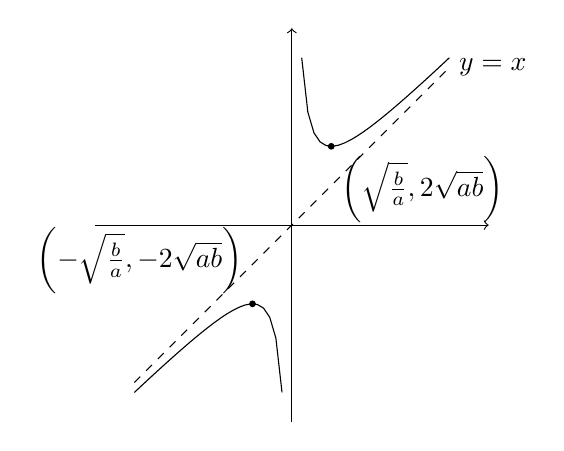
\begin{tikzpicture}[scale=0.5]
			    		\draw[black, ->] (-5,  0)--( 5,  0);
			    		\draw[black, ->] ( 0, -5)--( 0,  5);
			    		\draw[black, domain=-4:-0.25] plot(\x,\x + 1 / \x);
						\draw[black, domain=0.25:4] plot(\x,\x + 1 / \x);
						\draw[black, dashed, domain=-4:4] plot(\x, \x) node[anchor = west] at (4, 4) {$y=x$};
						\filldraw[black] (-1, -2) circle (2pt) node[anchor=south east] {$\left(-\sqrt{\frac{b}{a}}, -2\sqrt{ab}\right)$};
						\filldraw[black] ( 1,  2) circle (2pt) node[anchor=north west] {$\left(\sqrt{\frac{b}{a}}, 2\sqrt{ab}\right)$};
			    	\end{tikzpicture}
			    	&
			    	\begin{tikzpicture}[scale=0.5]
			    		\draw[black, ->] (-5,  0)--( 5,  0);
			    		\draw[black, ->] ( 0, -5)--( 0,  5);
			    		\draw[black, domain=-4:-0.25] plot(\x,\x - 1 / \x);
						\draw[black, domain=0.25:4] plot(\x,\x - 1 / \x);
						\draw[black, dashed, domain=-4:4] plot(\x, \x) node[anchor = west] at (4, 4) {$y=x$};
						\filldraw[black] (-1, 0) circle (2pt) node[anchor=south east] {$-\sqrt{-\frac{b}{a}}$};
						\filldraw[black] ( 1, 0) circle (2pt) node[anchor=north west] {$\sqrt{-\frac{b}{a}}$};
			    	\end{tikzpicture}
			    	\\\\
			    	a<0, b<0&a<0, b>0\\
			    	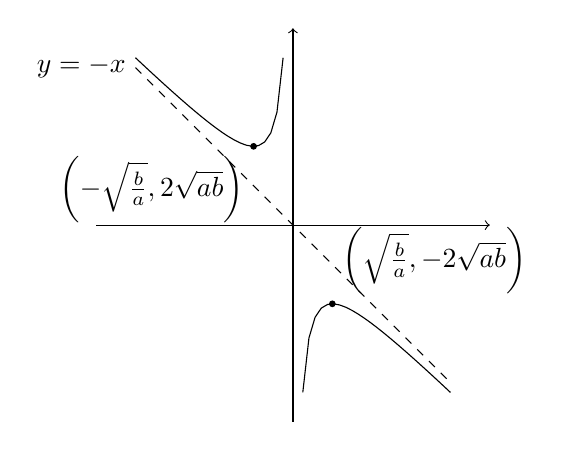
\begin{tikzpicture}[scale=0.5]
			    		\draw[black, ->] (-5,  0)--( 5,  0);
			    		\draw[black, ->] ( 0, -5)--( 0,  5);
			    		\draw[black, domain=-4:-0.25] plot(\x,-\x - 1 / \x);
						\draw[black, domain=0.25:4] plot(\x,-\x - 1 / \x);
						\draw[black, dashed, domain=-4:4] plot(\x, -\x) node[anchor = east] at (-4, 4) {$y=-x$};
						\filldraw[black] (-1,  2) circle (2pt) node[anchor=north east] {$\left(-\sqrt{\frac{b}{a}}, 2\sqrt{ab}\right)$};
						\filldraw[black] ( 1, -2) circle (2pt) node[anchor=south west] {$\left(\sqrt{\frac{b}{a}}, -2\sqrt{ab}\right)$};
			    	\end{tikzpicture}
			    	&
			    	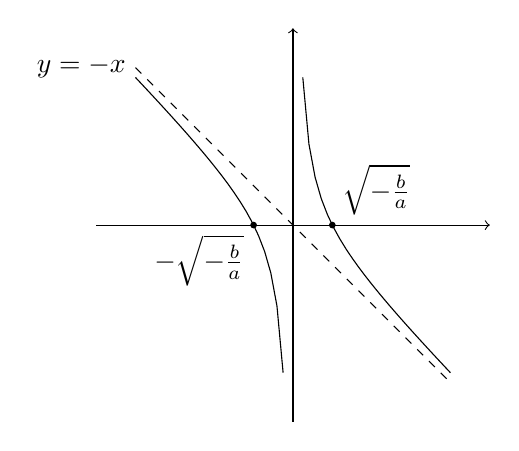
\begin{tikzpicture}[scale=0.5]
			    		\draw[black, ->] (-5,  0)--( 5,  0);
			    		\draw[black, ->] ( 0, -5)--( 0,  5);
			    		\draw[black, domain=-4:-0.25] plot(\x,-\x + 1 / \x);
						\draw[black, domain=0.25:4] plot(\x,-\x + 1 / \x);
						\draw[black, dashed, domain=-4:4] plot(\x, -\x) node[anchor = east] at (-4, 4) {$y=-x$};
						\filldraw[black] (-1, 0) circle (2pt) node[anchor=north east] {$-\sqrt{-\frac{b}{a}}$};
						\filldraw[black] ( 1, 0) circle (2pt) node[anchor=south west] {$\sqrt{-\frac{b}{a}}$};
			    	\end{tikzpicture}
					\end{array}
					$$
				~\\

				\textbf{例四}: 已知函数$f(x)=x^2+\dfrac{a}{x} (x\neq 0, a\in \mathbb{R})$. 若$a=2$, 解不等式$f(x)-f(x-1)>2x-1.$
					~\\

					\begin{align*}
						f(x) - f(x-1) = 2x-1 + \frac{2[(x-1)-x]}{x(x-1)} &> 2x-1\\
						\frac{-2}{x(x-1)} &> 0\\
						x(x-1) &< 0\\
						x &\in (0, 1).\\
					\end{align*}

					\textbf{\textcolor{red}{总结: 正常计算即可.}}

				~\\

				\textbf{例五}: 设$M=\{x|f(x)=0\}, N=\{x|g(x)=0\}$, 则方程$f(x)\cdot g(x) = 0$解集为 A. $M\cap N$ B. $M\cup N$ C. $M \text{ or } N$ D. 不确定.
					~\\

					$D_f = \{1, 2, 4\}, M = \{1, 2\}; D_g = \{2, 3, 4\}, N = \{2, 3, 4\}. f(x) g(x) = 0 \Rightarrow x \in \{2, 4\}.$

					\begin{align*}
					\{x|f(x)\cdot g(x) = 0\} &= \left(\{x|f(x) = 0\} \cap D_g\right) \cup \left(\{x|g(x) = 0\} \cap D_f\right)\\
					&= \left(M \cap D_g \right) \cup \left(N \cap D_f \right)\\
					&= \left[M \cup \left(N \cap D_f \right)\right] \cap \left[D_g \cup \left(N \cap D_f \right)\right]\\
					&= \left[\left(M \cup N\right) \cap \left(M \cup D_f\right) \right] \cap \left[\left(D_g \cup N\right) \cap \left(D_g \cup D_f\right)\right]\\
					&= (M\cup N)\cap D_f \cap D_g.
					\end{align*}

					\textbf{\textcolor{red}{总结: 注意函数定义域对函数的运算的影响.}}

				~\\

				\textbf{例六}: 
					$$
					\begin{array}{cc}
					y=|x+1|+|x-2|&y=|x+1|+|x-1|+|x-2|\\
					\begin{tikzpicture}[scale=0.5]
			    		\draw[black, ->] (-5,  0)--( 5,  0);
			    		\draw[black, ->] ( 0, -1)--( 0,  5);
			    		\draw[black] (-3, 7)--(-1, 3)--(2, 3)--(4, 7);
						\filldraw[black] (-1, 3) circle (2pt) node[anchor=north east] {$(-1, 3)$};
						\filldraw[black] ( 2,  3) circle (2pt) node[anchor=north west] {$(2, 3)$};
			    	\end{tikzpicture}
			    	&
			    	\begin{tikzpicture}[scale=0.5]
			    		\draw[black, ->] (-5,  0)--( 5,  0);
			    		\draw[black, ->] ( 0, -1)--( 0,  5);
			    		\draw[black] (-2, 8)--(-1, 5)--(1, 3)--(2, 4)--(3, 7);
						\filldraw[black] (-1, 5) circle (2pt) node[anchor=north east] {$(-1, 5)$};
						\filldraw[black] (1, 3) circle (2pt) node[anchor=north] {$(1, 3)$};
						\filldraw[black] (2, 4) circle (2pt) node[anchor=north west] {$(2, 4)$};
			    	\end{tikzpicture}
			    	\\\\
			    	y=|x+2|+|x+1|+|x-1|+|x-2|&\\
			    	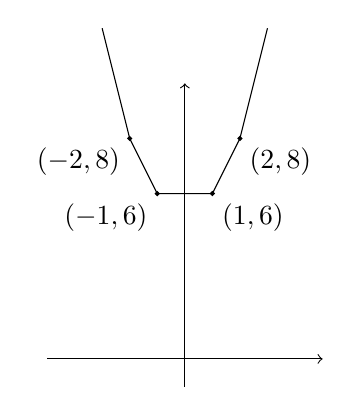
\begin{tikzpicture}[scale=0.35]
			    		\draw[black, ->] (-5,  0)--( 5,  0);
			    		\draw[black, ->] ( 0, -1)--( 0,  10);
			    		\draw[black] (-3, 12)--(-2, 8)--(-1, 6)--(1, 6)--(2, 8)--(3, 12);
						\filldraw[black] (-2, 8) circle (2pt) node[anchor=north east] {$(-2, 8)$};
						\filldraw[black] (-1, 6) circle (2pt) node[anchor=north east] {$(-1, 6)$};
						\filldraw[black] (1, 6) circle (2pt) node[anchor=north west] {$(1, 6)$};
						\filldraw[black] (2, 8) circle (2pt) node[anchor=north west] {$(2, 8)$};
			    	\end{tikzpicture}
			    	&
			    	\end{array}
					$$

					\textbf{\textcolor{red}{总结: $y=|x-x_1|+|x-x_2|+\cdots+|x-x_n|$函数的图像及性质: (1) 呈U型; (2) 当$n$为偶数, 中间两零点间为平底; (3) 当$n$为奇数, 尖底, 中间一个零点取最小值.}}

				~\\

				\textbf{例七}: 已知函数$f(x)$满足$\forall x, y\in\mathbb{R}: f(x+y)-f(y)=(x+2y+1)x, f(0)=0.$
					\begin{enumerate}[label=(\arabic*)]
						\item 求$f(0)$.
							~\\

							令$x=1 y=0$, 有$0-f(0)=2$, 即$f(0)=-2$.
							~\\

						\item 若$f(x)+3>2x+a$恒成立, 求$a$的取值范围.
							~\\

							令$y=0$, 有$f(x)-f(0)=(x+1)x$, 有$f(x)=x^2+x-2$.

							即$x^2+x+1>2x+a$恒成立, 即$x^2-x+1-a>0$恒成立, 即$\Delta=1-4+4a<0$, 即$a<\dfrac{3}{4}.$

					\end{enumerate}

					\textbf{\textcolor{red}{总结: 带字母函数值恒成立问题一般使用赋特殊值法.}}

				~\\

				\textbf{例八}: 函数$y=f(x), D_f = \mathbb{R}$满足$\forall a,b \in \mathbb{R}: f(a+b)=f(a)+f(b)$, 且当$x>0$时, $f(x)<0$恒成立. 证明:
					\begin{enumerate}[label=(\arabic*)]
						\item $f(x)$为奇函数.
							~\\

							令$a=b=0$, $f(0)=f(0)+f(0) \Rightarrow f(0)=0.$

							令$a=x, b=-x$, $f(0)=f(x)+f(-x)=0 \Rightarrow f(x)=-f(-x),$

							即$f(x)$为$\mathbb{R}$上的奇函数.
							~\\

						\item $y=f(x)$是$\mathbb{R}$上的严格减函数.
							~\\

							令$x_1 > x_2$, $f(x_1) - f(x_2) = f(x_1 - x_2) + f(x_2) - f(x_2) = f(x_1 - x_2).$

							$\because x_1 - x_2 > 0 \therefore f(x_1 - x_2) < 0 \therefore f(x_1) < f(x_2) \therefore$ 严格减函数.

					\end{enumerate}

					\textbf{\textcolor{red}{总结: 带字母函数值恒成立问题一般使用赋特殊值法.}}

				~\\

				\textbf{复合函数的单调性判定原则}: \textbf{同增异减}. \textbf{e.g.} $y=f[g(x)], f(x)=2x+1, g(x)=x^2. f(x)$在$\mathbb{R}$上严格单调递增, $g(x)$在$(-\infty, 0]$上严格单调递减, 在$[0, +\infty)$上严格单调递增, 故$f[g(x)]$在$(-\infty, 0]$上严格单调递减, 在$[0, +\infty)$上严格单调递增. \textbf{e.g.} $f(x)=\dfrac{1}{x^2}$, 令$p(x)=x^2, q(t)=\dfrac{1}{t}$, 则$p(x)$在$(-\infty, 0)$上严格单调递减, 在$(0, +\infty)$上严格单调递增, $q(t)$在$(-\infty, 0)$和$(0, +\infty)$上分别严格单调递减, 故$f(x)$在$(-\infty, 0)$上严格单调递增, 在$(0, +\infty)$上严格单调递减.

			\subsubsection{函数的最值}
				\textbf{最值的定义}: 函数$y=f(x)$在$x_0$处的函数值是$f(x_0)$. 对于定义域内任意给定的$x$, 如果$$f(x)\geq f(x_0)$$都成立, 那么$f(x_0)$就叫做函数$y=f(x)$的\textbf{最小值}, 记作$$y_{\min}=f(x)_{\min}=f(x_0);$$

				相反, 如果$$f(x)\leq f(x_0)$$都成立, 那么$f(x_0)$就叫做函数$y=f(x)$的\textbf{最大值}, 记作$$y_{\max}=f(x)_{\max}=f(x_0).$$

				最大值与最小值统称为\textbf{最值}.

				\textbf{单调区间上的极值问题}: 对于定义在闭区间$[a, b]$上的单调函数$y=f(x)$, 它的最大值和最小值\textbf{一定能在区间的端点$a$和$b$处取到}.

				\textbf{二次函数在闭区间上的最值问题}: 考虑$f(x)=a(x-m)^2+n (a>0)$在$[h, k]$上的最值,

				\begin{enumerate}[label=$\arabic*^{\circ}$]
					\item $m\in[h,k]$, 有$y_{\min}=n, y_{\max}=\max\left\{f(h), f(k)\right\}$;
					\item $m\notin[h,k]$, 有$y_{\min}=\min\left\{f(h), f(k)\right\}, y_{\max}=\max\left\{f(h), f(k)\right\}$.
				\end{enumerate}

				结论:

				\begin{enumerate}[label=$\arabic*^{\circ}$]
					\item 抛物线开口向上:

						求最小值, 分对称轴在区间左, 中, 右三段;

						求最大值, 分对称轴在区间中点的左, 右两段.

					\item 抛物线开口向下:

						求最小值, 分对称轴在区间中点的左, 右两段;

						求最大值, 分对称轴在区间左, 中, 右三段.
				\end{enumerate}

				求最值, 分四段.

				~\\

				\textbf{例一}: 求$y=x^2-2x-3, x\in[0, 3]$的最值.
					~\\

					对称轴: 直线$x=1$.

					$$
					\begin{tikzpicture}[scale=0.75]
			    		\draw[black, ->] (-1,  0)--( 5,  0);
			    		\draw[black, ->] ( 0, -5)--( 0,  1);
			    		\draw[black, domain=0:3] plot(\x, \x * \x - 2 * \x - 3);
			    		\draw[black, dashed] ( 1, 0.5)--( 1, -5);
						\filldraw[black] (3, 0) circle (2pt) node[anchor=south west] {$3$};
						\filldraw[black] (0, -3) circle (2pt) node[anchor=east] {$-3$};
			    	\end{tikzpicture}$$

			    	当$x=1$时, $y_{\min}=-4; $当$x=3$时, $y_{\max}=0.$

					\textbf{\textcolor{red}{总结: 定轴定区间的二次函数最值问题比较简单.}}

				~\\

				\textbf{含参变量的二次函数最值问题}:

				\textbf{例二}: 求$y=x^2+2ax+3$在$x\in[-2, 2]$的最值.
					~\\

					$y=(x+a)^2+3-a^2. $当$x=-2$时, $y=7-4a$; 当$x=2$时, $y=7+4a$.

					\begin{enumerate}[label=$\arabic*^{\circ}$]
						\item $-a\leq -2,$ 即$a\geq 2$,

							当$x=-2$时, $y_{\min}=7-4a$;

							当$x=2$时, $y_{\max}=7+4a$.

						\item $-2<-a\leq 0,$ 即$0\leq a<2$,

							当$x=-a$时, $y_{\min}=3-a^2$;

							当$x=2$时, $y_{\max}=7+4a$.

						\item $0<-a\leq 2,$ 即$-2\leq a<0$,

							当$x=-a$时, $y_{\min}=3-a^2$;

							当$x=-2$时, $y_{\max}=7-4a$.

						\item $-a>2,$ 即$a<-2$,

							当$x=2$时, $y_{\min}=7+4a$;

							当$x=-2$时, $y_{\max}=7-4a$.
					\end{enumerate}

					综上,

					$$
					y_{\min}=\left\{\begin{array}{rl}7-4a,& a\geq 2\\ 3-a^2,& -2<a<2\\ 7+4a, &a\leq -2,\end{array}\right.
					$$

					$$
					y_{\max}=\left\{\begin{array}{rl}7+4a,& a\geq 0\\ 7-4a, &a<0. \end{array}\right.
					$$

					\textbf{\textcolor{red}{总结: 动轴定区间问题需分类讨论.}}

				~\\

				\textbf{例三}: 求函数$y=x^2-2x-3$在$x\in[k, k+2]$的最值.
					~\\

					对称轴: 直线$x=1$. 当$x=k$时, $y=k^2-2k-3$; 当$x=k+2$时, $y=k^2+2k-3$.

					\begin{enumerate}[label=$\arabic*^{\circ}$]
						\item $1\leq k, $即$k\geq 1$,

							当$x=k$时, $y_{\min}=k^2-2k-3$;

							当$x=k+2$时, $y_{\max}=k^2+2k-3$.

						\item $k<1\leq k+1, $即$0\leq k<1$,

							当$x=1$时, $y_{\min}=-4$;

							当$x=k+2$时, $y_{\max}=k^2+2k-3$.

						\item $k+1<1\leq k+2, $即$-1\leq k<0$,

							当$x=1$时, $y_{\min}=-4$;

							当$x=k$时, $y_{\max}=k^2-2k-3$.

						\item $1>k+2, $即$k<-1$,

							当$x=k+2$时, $y_{\min}=k^2+2k-3$;

							当$x=k$时, $y_{\max}=k^2-2k-3$.
					\end{enumerate}

					综上,

					$$
					y_{\min}=\left\{\begin{array}{rl}k^2-2k-3,& k\geq 1,\\ -4,& -1\leq k<1,\\ k^2+2k-3, &k<-1,\end{array}\right.
					$$

					$$
					y_{\max}=\left\{\begin{array}{rl}k^2+2k-3,& k\geq 0\\ k^2-2k-3, &k<0. \end{array}\right.
					$$

					\textbf{\textcolor{red}{总结: 定轴动区间问题需分类讨论.}}

				~\\

				\textbf{例四}: 求$y=x^2-2x-3$在$x\in[-3, m]$函数的最值.
					~\\

					$y=(x-1)^2-4$, 对称轴为直线$x=1$.

					\begin{enumerate}[label=$\arabic*^{\circ}$]
						\item $-3<m<1$, 有

							$x=-3$, $y_{\max}=12;$

							$x=m$, $y_{\min}=m^2-2m-3.$

						\item $1\leq m<5$, 有

							$x=-3$, $y_{\max}=12;$

							$x=1$, $y_{\min}=-4.$

						\item $m\geq 5$, 有

							$x=m$, $y_{\max}=m^2-2m-3;$

							$x=1$, $y_{\min}=-4.$

					\end{enumerate}

					\textbf{\textcolor{red}{总结: 定轴动区间问题需分类讨论.}}

				~\\

				\textbf{例五}: $x\in[-1, 1]$时, $f(x)=-x^2-ax+2$.
					~\\

					$f(x)=-\left(x+\frac{a}{2}\right)$, 对称轴为直线$x=-\frac{a}{2}$.

					\begin{enumerate}[label=(\arabic*)]
						\item 若最小值为$-1$, 求$a$的取值范围.
							~\\

							\begin{enumerate}[label=$\arabic*^{\circ}$]
								\item $-\frac{a}{2}\leq0$即$a\geq0$,

									$$f(x)_{\min}=f(1)=-1-a+2=-a, a=2.$$

								\item $-\frac{a}{2}>0$即$a<0$,

									$$f(x)_{\min}=f(-1)=-1+a+2=-1, a=-2.$$

							\end{enumerate}

							综上, $a=\pm 2.$

						~\\

						\item 若最大值为$\frac{11}{4}$, 求$a$的取值范围.
							~\\

							\begin{enumerate}[label=$\arabic*^{\circ}$]
								\item $-\frac{a}{2}<-1$即$a>2$,

									$$f(x)_{\max}=f(-1)=-1+a+2=\frac{11}{4}, a=\frac{7}{4} \text{(舍)}.$$

								\item $-\frac{a}{2}>1$即$a<-2$,

									$$f(x)_{\max}=f(1)=-1-a+2=\frac{11}{4}, a=-\frac{7}{4} \text{(舍)}.$$

								\item $-1\leq -\frac{a}{2}\leq 1$即$-2\leq a\leq 2$,

									$$f(x)_{\max}=f\left(-\frac{a}{2}\right)=\frac{a^2}{4}+2=\frac{11}{4}, a=\pm \sqrt{3}.$$

							\end{enumerate}

							综上, $a=\pm \sqrt{3}.$

					\end{enumerate}

					\textbf{\textcolor{red}{总结: 已知最值反向求参数本质上为分类讨论求最值然后解方程.}}

				~\\

				\textbf{不等式恒成立问题}: 二次函数$>0, <0$恒成立: 在$\mathbb{R}$上, 考虑二次项系数与判别式; 在某给定区间上, 讨论最值 or 参变分离.

				~\\

				\textbf{例六}: $x^2-2mx+2m+1>1$在$x\in[0, 1]$时恒成立, 求$m$的取值范围.
					~\\

					$$2m(x-1)<x^2+1.$$

					当$x=1$, 显然符合.

					当$x\in [0, 1)$, 有

					$$2m>\frac{x^2+1}{x-1}.$$

					令$x-1=t\in[-1, 0)$, 有

					$$2m>\frac{t^2+2t+2}{t}.$$

					有

					$$u(t)=\frac{t^2+2t+2}{t}=t+\frac{2}{t}+2\leq -2\sqrt{2}+2,$$

					等号成立当且仅当$t=-\sqrt{2} \notin [-1, 0)$.

					$\because$ $u(t)$在$[-1, 0)$严格减

					$\therefore$ $u(t)_{\max}=u(-1)=-1$

					$\therefore$ $2m>-1$即$m>-\dfrac{1}{2}.$	

					\textbf{\textcolor{red}{总结: 可以使用参变分离法进行恒成立问题的分析.}}

				~\\

				\textbf{例七}: 二次函数$f(x)=ax^2+bx (a, b\text{为常数且}a\neq 0)$, $f(2)=0$且$f(x)=x$有等根.
					\begin{enumerate}[label=(\arabic*)]
						\item 求$f(x)$解析式.
							~\\

							$$f(x)=-\frac{1}{2} x^2 + x = -\frac{1}{2} (x-1)^2 + \frac{1}{2}.$$

							~\\

						\item 是否存在$m, n (m<n)$使$f(x)$的定义域和值域分别为$[m, n]$和$[2m, 2n]$?
							~\\

							$$f(x) \leq \frac{1}{2} \Rightarrow n\leq \frac{1}{4}\Rightarrow f(x)\text{在}[m, n]\text{上严格增} \Rightarrow \left\{\begin{array}{rcl}f(m)&=&2m\\f(n)&=&2n\end{array}\right. \Rightarrow \left\{\begin{array}{rcl}m&=&2\\n&=&0\end{array}\right..$$

							~\\

						\item [推广] $g(x)=-\dfrac{1}{2}x^2+ax$, 是否存在$m, n (m<n)$使$g(x)$的定义域和值域分别为$[m, n]$和$[2m, 2n]$?
							~\\

							此时需要对$g(x)$的对称轴进行分类讨论, 不多作赘述.
							
					\end{enumerate}

					\textbf{\textcolor{red}{总结: 二次函数的极值问题的分类讨论需注意逻辑的严密性.}}

				~\\

				\textbf{例十}: 设$a\in\mathbb{R}$, $f(x)=x^2+|x-a|+1$, $x\in\mathbb{R}$.
					\begin{enumerate}[label=(\arabic*)]
						\item 讨论$f(x)$奇偶性.
							~\\

							当$a=0$, $f(x)=x^2+|x|+1$, $D=\mathbb{R}$, $f(-x)=(-x^2)+|-x|+1=-f(x)$, 奇函数.

							当$a\neq 0$, $f(a)=a^2+1$, $f(-a)=a^2+2|a|+1$, 非奇非偶.

							~\\

						\item 求$f(x)$最小值.
							~\\

							$$f(x)=\left\{\begin{array}{rl}x^2+x-a+1, &x\geq a,\\x^2-x-a+1, &x<a.\end{array}\right.$$

							$x\geq a$对称轴为直线$x=-\dfrac{1}{2}$, $x<a$对称轴为直线$x=\dfrac{1}{2}$.

							\begin{enumerate}[label=$\arabic*^{\circ}$]
								\item $a\leq -\dfrac{1}{2}$, $f(x)_{\min} = f\left(-\dfrac{1}{2}\right)=\dfrac{3}{4}-a$.
								\item $-\dfrac{1}{2}<a\leq\dfrac{1}{2}$, $f(x)_{\min} = f(a) = a^2+1$.
								\item $a>\dfrac{1}{2}$, $f(x)_{\min}=f\left(\dfrac{1}{2}\right)=a+\dfrac{3}{4}$.
							\end{enumerate}
							
					\end{enumerate}

					\textbf{\textcolor{red}{总结: 二次函数的极值问题的分类讨论需注意逻辑的严密性.}}

				~\\

				\textbf{一次分式函数的极值}: $y=\dfrac{cx+d}{ax+b} (a\neq 0, \dfrac{c}{a} \neq \dfrac{d}{b})$, 将分子换元分离整系数.

				~\\

				\textbf{例一}: 求$y=\dfrac{2x-1}{3-x}$的值域.
					~\\

					$$y=\frac{1-2x}{x-3}=\frac{-2(x-3)-5}{x-3}=-2+\frac{-5}{x-3}.$$

					$$
					\begin{tikzpicture}[scale=0.5]
			    		\draw[black, ->] (-3,  0)--( 8,  0);
			    		\draw[black, ->] (0, -7)--( 0, 3);
			    		\draw[black, domain=-2.5:2] plot(\x, {(2*\x-1)/(3-\x)});
			    		\draw[black, domain=4:7.5] plot(\x, {(2*\x-1)/(3-\x)});
			    		\draw[black, dashed] (-2.75, -2)--(7.75, -2) node[right] {$y=-2$};
			    		\draw[black, dashed] (3, -6.75)--(3, 2.75) node[above] {$x=3$};
			    	\end{tikzpicture}$$

			    	故值域为$(-\infty, -2)\cup(-2, +\infty).$

					\textbf{\textcolor{red}{总结: $y=\dfrac{cx+d}{ax+b} (a\neq 0, \dfrac{c}{a} \neq \dfrac{d}{b})$, 定义域$D=\left\{x|x\neq\dfrac{b}{a}\right\}$, 值域$R=\left\{y|y\neq\dfrac{c}{a}\right\}$.}}

				~\\

				\textbf{二次分式的极值}: $y=x+\dfrac{a}{x}, y=\dfrac{a_1x^2+b_1x+c_1}{a_2x^2+b_2x+c_2}.$

				~\\

				\textbf{例二}: 求函数$y=\dfrac{5}{2x^2-4x+3}$的值域.
					~\\

					$$y=\frac{5}{2(x-2)^2+1}\in(0, 5].$$

					\textbf{\textcolor{red}{总结: 分子常数, 分母二次, 分母配方.}}

				~\\

				\textbf{例三}: 求函数$y=\dfrac{1-x^2}{1+x^2}$的值域.
					~\\

					$$x^2=\frac{1-y}{y+1}\geq 0\Rightarrow y\in(-1, 1].$$

					\textbf{\textcolor{red}{总结: 分子分母各项齐次, 考虑使用二次方恒非负 (注意定义域问题).}}

				~\\

				\textbf{例四 (1)}: 求$y=\dfrac{x}{x^2+4x+5}$的值域.
					~\\

					\textbf{法一: 转换为双勾函数处理}.

					\begin{enumerate}[label=$\arabic*^{\circ}$]
						\item $x=0$时, $y=0$.
						\item $x\neq 0$时, 有:

							$$y=\frac{1}{x+\frac{5}{x}+4}.$$

							有

							$$x+\frac{5}{x} \geq 2\sqrt{5} \text{ or } x+\frac{5}{x} \leq -2\sqrt{5},$$

							故

							$$y\in\left[-\frac{2+\sqrt{5}}{2}, 0\right)\cup\left(0, \frac{\sqrt{5}-2}{2}\right].$$

					\end{enumerate}

					综上, $y\in \left[-\dfrac{2+\sqrt{5}}{2}, \dfrac{\sqrt{5}-2}{2}\right]$.

					\textbf{法二: $\Delta$法}, 适用条件: (1) 二次分式 (2) 定义域为自然定义域. 将函数值域问题转化为方程有解问题.

					$$y=\frac{x}{x^2+4x+5}\text{的值域} \Leftrightarrow \text{关于}x\text{的方程}yx^2+(4y-1)x+5y=0\text{有解}.$$

					\begin{enumerate}[label=$\arabic*^{\circ}$]
						\item $y=0$时, 有解.
						\item $y\neq 0$时, 有:

							$$\Delta = (4y-1)^2-20y^2=-4y^2-8y+1\geq 0,$$

							有

							$$y\in\left[-\frac{2+\sqrt{5}}{2}, 0\right)\cup\left(0, \frac{\sqrt{5}-2}{2}\right].$$

					\end{enumerate}

					综上, $y\in \left[-\dfrac{2+\sqrt{5}}{2}, \dfrac{\sqrt{5}-2}{2}\right]$.

					\textbf{\textcolor{red}{总结: 限定区间用法一, 不限定区间用法二 (法二适用于一切二次分式为通法).}}

				~\\

				\textbf{例四 (1)}: 求$y=2x+\frac{8}{x} (0<x\leq 1)$的值域.
					~\\

					$(0, 1]$上有$y$严格减, 故$y\in[10, +\infty).$

					\textbf{\textcolor{red}{总结: 函数在指定区间上存在单调性的可以直接利用单调性解决.}}

				~\\

				\textbf{根式的最值}:

				~\\

				\textbf{例五}: 求$y=2x-3+\sqrt{13-4x}$的最值.
					~\\

					令$t=\sqrt{13-4x}\in[0, +\infty),$有

					$$x=\frac{13-t^2}{4},$$

					故有

					\begin{align*}
						y &= \frac{13-t^2}{2}-3+t\\
						  &= -\frac{1}{2} t^2 + t + \frac{7}{2}\\
						  &= -\frac{1}{2} (t-1)^2 + 4,\\
					\end{align*}

					故有

					$$y_{\max}=4, y_{\min} \mathrm{\ D.N.E.}.$$

					\textbf{\textcolor{red}{总结: 根式函数的值域可以考虑将根式换元将其变为整式.}}

				~\\

				\textbf{例六}: 求$y=2x-\sqrt{1-x}$的最大值.
					~\\

					$D=(-\infty, 1]$, $f(x)$在$D$上单调增,

					故$f(x)_{\max}=f(1)=2.$

					\textbf{\textcolor{red}{总结: 单调的根式函数可以直接利用单调性.}}

			\subsubsection{函数的周期性}

				\textbf{周期函数的定义}: 对于函数$y=f(x)$, 如果存在一个非零常数$T$, 使得当$x$取其定义域$D$中的任意值时, 有$x+T \in D$, 且成立$$f(x+T)=f(x),$$ 那么函数$y=f(x)$就叫作\textbf{周期函数}, 而这个非零常数$T$就叫做函数$y=f(x)$的一个\textbf{周期}.

				\textbf{最小正周期}: 对于一个周期函数$y=f(x)$, 如果它在所有周期中存在一个最小正数, 那么这个最小正数就叫作函数$y=f(x)$的\textbf{最小正周期}.


				\textbf{例}: 函数$f(x)$对于任意实数$f(x)$满足条件:

					$$f(x+2)=\frac{1}{f(x)},$$

					且有$f(0)=1, f(1)=-5.$

					\begin{enumerate}[label=(\arabic*)]
						\item 计算$f(2), f(4), f(6), f(8)$的值, 并猜想$f(2n)$的结果, 其中$n \in \mathbb{N}.$
						\item 计算$f(3), f(5), f(7), f(9)$的值, 并猜想$f(2n-1)$的结果, 其中$n \in \mathbb{N}.$
						\item 试证明(1), (2)所猜想的结果.
					\end{enumerate}
					~\\

					\begin{enumerate}[label=(\arabic*)]
						\item 计算$f(2), f(4), f(6), f(8)$的值, 并猜想$f(2n)$的结果, 其中$n \in \mathbb{N}.$

							$$f(2)=\frac{1}{f(2-2)}=\frac{1}{f(0)}=\frac{1}{1}=1, f(4)=\frac{1}{f(4-2)}=\frac{1}{f(2)}=\frac{1}{1}=1,$$

							$$f(6)=\frac{1}{f(6-2)}=\frac{1}{f(4)}=\frac{1}{1}=1, f(8)=\frac{1}{f(8-2)}=\frac{1}{f(6)}=\frac{1}{1}=1,$$

							猜想:

							$$f(2n)=1, n \in \mathbb{N}. \eqno{(1)}$$

						\item 计算$f(3), f(5), f(7), f(9)$的值, 并猜想$f(2n-1)$的结果, 其中$n \in \mathbb{N}.$

							$$f(3)=\frac{1}{f(3-2)}=\frac{1}{f(1)}=\frac{1}{-5}=-\frac{1}{5}, f(5)=\frac{1}{f(5-2)}=\frac{1}{f(3)}=\frac{1}{-\frac{1}{5}}=-5,$$

							$$f(7)=\frac{1}{f(7-2)}=\frac{1}{f(5)}=\frac{1}{-5}=-\frac{1}{5}, f(9)=\frac{1}{f(9-2)}=\frac{1}{f(7)}=\frac{1}{-\frac{1}{5}}=-5,$$

							猜想:

							$$f(2n-1)=
							\left\{
							\begin{array}{rl}
							-5,& n\text{是奇数},\\
							\displaystyle -\frac{1}{5}, &n\text{是偶数}.\\
							\end{array}
							\right.
							\eqno{(2)}
							$$

						\item 试证明 (1), (2) 所猜想的结果.

							\textbf{下证 (1) 式成立:}

								考虑$n=0$, 有

								$$f(2\times0)=f(0)=1$$

								符合 (1) 式.

								假设 (1) 式对$n=k$成立, 下证其对$n=k+1$成立.

								$$f[2(k+1)]=f(2k+2)=\frac{1}{f(2k+2-2)}=\frac{1}{f(2k)}=\frac{1}{1}=1$$

								成立.

								由第一数学归纳法, (1) 式成立.

							\textbf{下证 (2) 式成立:}

								考虑$n=0$, 有

								$$f(1)=\frac{1}{f(1-2)}=\frac{1}{f(-1)}=\frac{1}{f(2\times 0-1)}=-5 \Rightarrow f(2\times0-1)=f(-1)=-\frac{1}{5}$$

								符合 (2) 式.

								考虑$n=1$, 有

								$$f(2\times 1-1)=f(1)=-5$$

								符合 (2) 式.

								假设 (2) 式对$n=2k$成立, 下证其对$n=2k+2$成立.

								$$f[2(2k+2)-1]=f(4k+3)=\frac{1}{f(4k+3-2)}=\frac{1}{f(4k+1)}=\frac{1}{\frac{1}{f(4k+1-2)}}=\frac{1}{\frac{1}{f(4k-1)}}=f(4k-1)=f[2(2k)-1]=-\frac{1}{5}$$

								成立.

								假设 (2) 式对$n=2k+1$成立, 下证其对$n=2k+3$成立.

								$$f[2(2k+3)-1]=f(4k+5)=\frac{1}{f(4k+5-2)}=\frac{1}{f(4k+3)}=\frac{1}{\frac{1}{f(4k+3-2)}}=\frac{1}{\frac{1}{f(4k+1)}}=f(4k+1)=f[2(2k+1)-1]=-5$$

								成立.

								由第一数学归纳法, (2) 式成立.

								\textbf{使用周期函数证明}:

								$$f(n+4)=f[(n+2)+2]=\frac{1}{f(n+2)}=f(x),$$

								即该函数存在周期$T=4$.

								又$\because f(0)=1, f(1)=-5, f(-1)=\displaystyle-\frac{1}{5}$

								$\therefore$......得证.
					\end{enumerate}

					\textbf{\textcolor{red}{总结: (1) $\displaystyle f(x+k)=\frac{1}{f(x)} \Rightarrow $周期$T=2k$ (2) 周期法证明和数学归纳法证明都是十分有效的方案.}}

		\newpage
		\subsection{函数的应用}
			\subsubsection{函数关系的建立}

				注意函数的定义域.

				~\\

				\textbf{例一}: 已知$$f\left(1+\frac{1}{x}\right)=\frac{1}{x^2}-1,$$

					求函数$y=f(x)$.
					~\\

					令$\displaystyle t=1+\frac{1}{x} (t\neq 1),$

					则$\displaystyle \frac{1}{x}=t-1, \frac{1}{x^2}=(t-1)^2.$

					有$\displaystyle f(t)=(t-1)^2-1=t^2-26, t\neq 1.$

					即$\displaystyle y=f(x)=x^2-2x, x\in(-\infty, 1)\cup(1, +\infty).$

					\textbf{\textcolor{red}{总结: (1) 换元法是解决建立函数关系相关问题的一个好方法 (2) 换元时注意变量的取值范围.}}

				~\\

				\textbf{例二}: 已知$$f\left(x+\frac{1}{x}\right)=x^2+\frac{1}{x^2},$$

					求函数$y=f(x)$.
					~\\

					令$\displaystyle t=x+\frac{1}{x}\in(-\infty, 2]\cup[2, +\infty),$

					则$\displaystyle x^2+\frac{1}{x^2}=t^2-2,$

					有$\displaystyle f(t)=t^2=2, t\in(-\infty, -2]\cup[2, +\infty),$

					即$\displaystyle y=f(x)=x^2-2, x\in(-\infty, -2]\cup[2, +\infty).$

					\textbf{\textcolor{red}{总结: 可利用基本不等式解决变量的取值范围.}}

				~\\

				\textbf{例三}: 函数$f(x)=2x-1$, $\displaystyle g(x)=\left\{\begin{array}{rl}x^2,&x\geq 0,\\-1,&x<0\end{array}\right.$, 求$f[g(x)]$和$g[f(x)]$的解析式.
					~\\

					\textbf{下求:} $f[g(x)]$的解析式.

					当$x\geq 0$时, $g(x)=x^2$, $f[g(x)]=f(x^2)=2x^2-1$;

					当$x< 0$时, $g(x)=-1$, $f[g(x)]=f(-1)=-3$.

					$\displaystyle \therefore f[g(x)]=\left\{\begin{array}{rl}2x^2-1,&x\geq 0,\\-3,&x<0.\end{array}\right.$
					~\\

					\textbf{下求:} $g[f(x)]$的解析式.

					当$f(x)\geq 0$即$\displaystyle x\geq \frac{1}{2}$时, $g[f(x)]=(2x-1)^2=4x^2-4x+1$;
					~\\

					当$f(x)< 0$即$\displaystyle x< \frac{1}{2}$时, $g[f(x)]=-1$.

					$\displaystyle \therefore g[f(x)]=\left\{\begin{array}{rl}4x^2-4x+1,&x\geq \displaystyle \frac{1}{2},\\\\-1,&x<\displaystyle \frac{1}{2}.\end{array}\right.$

					\textbf{\textcolor{red}{总结: 分段函数需注意“分段”的变量.}}

				~\\

				\textbf{例四}: 已知$f(x)$满足$2f(x)+f\displaystyle \left(\frac{1}{x}\right)=3x$. 求$f(x)$.
					~\\

					$$
					\left\{
					\begin{array}{rcl}
						2f(x)+\displaystyle f\left(\frac{1}{x}\right)&=&3x\\
						2\displaystyle f\left(\frac{1}{x}\right)+f(x)&=&\displaystyle\frac{3}{x}
					\end{array}
					\right.
					\Rightarrow f(x)=2x-\displaystyle \frac{1}{x}, x\in(-\infty, 0)\cup(0, +\infty).
					$$

					\textbf{\textcolor{red}{总结: 可以使用代入法求函数解析式.}}

			\subsubsection{用函数观点求解方程和不等式}
				\textbf{零点的定义}: 对于函数$f(x), x\in D$, 如果存在实数$c\in D$, 使得$$f(c)=0,$$ 就把$c$叫做该函数的零点.

				\textbf{零点与方程的解的联系}: 函数$y=f(x), x\in D$的零点, 就是方程$f(x)=0$在集合$D$中的解, 也是该函数$y=f(x)$的图像与$x$轴的交点的横坐标.

			\subsubsection{用二分法求函数的零点}
				\textbf{介值定理}: 如果在区间$[a, b]$上, 函数$y=f(x)$的图像是一段连续曲线, 并且$f(a)\cdot f(b)<0$, 那么$y=f(x)$在区间$(a, b)$上一定有零点.

				\textbf{零点与连续和端点异号的条件关系}: 函数在$[a, b]$上连续 and $f(a) \cdot f(b) \leq 0$ $\Rightarrow$ $y=f(x)$在$[a, b]$上有零点, $y=f(x)$在$[a, b]$上有零点 $\nRightarrow$ 函数在$(a, b)$上连续 and $f(a) \cdot f(b) \leq 0$.

				\textbf{零点数量和单调性的关系}: 函数在$[a, b]$上连续 and $f(a) \cdot f(b) \leq 0$ and $f(x)$在$[a, b]$上严格单调递增 $\Rightarrow$ $y=f(x)$在$(a, b)$上有唯一的零点.

				\textbf{二分法求零点的近似值}: 确定了$(a, b)$上一定有零点后, 将区间一分为二, 这两部分的区间中总有一个含有零点, 而含有零点的区间长度变为原来的一半. 反复执行这种 “一分为二” 的操作, 就能将零点限制在一个足够小的区间中, 从而容易求得其近似值了.

		\newpage
		\subsection{反函数}
			\textbf{反函数的定义}: 对于函数$y=f(x), x\in D$, 记其值域为$f(D)$. 如果对$f(D)$中的任意给定的一个值$y$, 在$D$中满足$f(x)=y$的$x$值只有一个, 那么由此得到的$x$关于$y$的函数叫做$y=f(x), x\in D$的\textbf{反函数}, 记作$x=f^{-1}(y), y\in f(D)$, 通常把该函数改写为:$$y=f^{-1}(x), x\in f(D).$$

			\textbf{反函数存在的充要条件}: 一个定义域为$D$的函数$y=f(x)$存在反函数, 当且仅当对于其值域$f(D)$中的\textbf{每一个值$y_0$}, 在定义域$D$中\textbf{仅存在一个$x_0$}, 满足$f(x_0)=y_0$. 简而言之, 如果$y=f(x)$在定义域$D$上\textbf{不同的$x$值所取到的函数值也不相同}, 那么$y=f(x)$就存在反函数.

			\textbf{反函数的存在性与单调性的关系}: 函数$y=f(x), x\in D$在定义域上严格增或严格减为该函数存在反函数的\textbf{充分非必要条件}.

			\textbf{原函数与反函数的关系}: $y=f(x), x\in D$与$y=f^{-1}(x), x\in f(D)$\textbf{互为反函数}. 函数$y=f^{-1} (x)$的定义域就是函数$y=f(x)$的值域, 函数$y=f^{-1} (x)$的值域就是函数$y=f(x)$的定义域.

			\textbf{原函数的图像与反函数的图像的关系}: 互为反函数的两函数的图像关于直线$y=x$成轴对称.

			\textbf{反函数和原函数单调性的关系}: 假设函数$y=f(x)$在$[a, b]$上被定义, 若$y=f(x)$在$[a, b]$上(严格)单调增(减), 则其反函数$y=f^{-1}(x)$在$[f(a), f(b)]$上(严格)单调增(减).

			\textbf{求反函数的一般步骤}: (1)求原函数$y=f(x)$在定义域$D$上的值域$f(D)$即为反函数$y=f^{-1}(x)$的定义域. (2) 在$y=f(x)$中用$y$表示$x$, 即改写为$x=f(y)$的形式. (3) 化简为$y=g(x)=f^{-1}(x)$. (4) 写出定义域$f(D)$.

			~\\

			\textbf{例一}: 求函数$$y=\left\{\begin{array}{rl}x^2-1,&0\leq x<1,\\x^2,&-1\leq x<0.\end{array}\right.$$的反函数.
				~\\

				分两段进行讨论.

				\begin{enumerate}[label=$\arabic*^{\circ}$]
					\item $0\leq x<1$时, $y\in[-1, 0)$, 得$x^2=y+1$, 即$x=\sqrt{y+1}$, 反函数即为$y=\sqrt{x+1}, x\in[-1, 0)$.

					\item $-1\leq x<0$时, $y\in(0, 1]$, 得$x=\sqrt{y}$, 即反函数为$y=\sqrt{x}, x\in(0, 1]$.	
				\end{enumerate}

				综上, 反函数为

				$$y=\left\{\begin{array}{rl}\sqrt{x+1},&x\geq -1,\\\sqrt{x},&0<x\leq 1.\end{array}\right.$$

				\textbf{\textcolor{red}{总结: 求解反函数一定要考虑值域和定义域的问题.}}

			~\\

			\textbf{反函数与原函数自变量的平移关系}: 函数$y=f(x), x\in D$的反函数为$y=f^{-1}(x), x\in f(D)$.

			下求$y=f(x+a)$的反函数.

			$$y=f(x+a)\Rightarrow x+a=f^{-1}(y) \Rightarrow x=f^{-1}(y)-a \Rightarrow \text{反函数为} y=f^{-1}(x)-a.$$

			下求$y=f^{-1}(x+a)$的反函数.

			$$y=f^{-1}(x+a)\Rightarrow x+a=f(y) \Rightarrow x=f(y)-a \Rightarrow \text{反函数为} y=f(x)-a.$$

			考察$y=f(x), y=f^{-1}(x), y=f(x+a), y=f^{-1}(x+a)$之间的关系:

			$$
			\begin{array}{ccc}
				y=f(x) & \xlongleftrightarrow[\text{关于直线$y=x$对称}]{\text{互为反函数}} & y=f^{-1}(x) \\
				\text{向左平移} \downarrow \text{$a$单位}& & \text{向左平移} \downarrow \text{$a$单位} \\
				y=f(x+a) & \xlongleftrightarrow[\text{关于直线$y=x+a$对称}]{\text{不一定互为反函数}} & y=f^{-1}(x+a)
			\end{array}
			$$

			~\\

			\textbf{例二}: 已知$f(x)=\dfrac{x+3}{2x-1}$, 函数$y=g(x)$的图像与$y=f^{-1}(x+1)$的图像关于$y=x$对称, 求$g(-1).$
				~\\

				$y=f^{-1}(x+1)$的反函数为$y=f(x)-1$, 故

				$$g(x)=f(x)-1=\frac{-x+4}{2x-1},$$
				
				有

				$$g(-1)=-\frac{5}{3}.$$

				\textbf{\textcolor{red}{总结: 反函数和原函数图像关于直线$y=x$对称的结论要熟记.}}

\end{document}